\documentclass[12pt]{article}
% include the pckage of the color%
\usepackage[usenames, dvipsnames]{color}
\usepackage[english]{babel}
\usepackage[utf8x]{inputenc}
\usepackage{amsmath}
\usepackage{graphicx}
\usepackage{array}

%define your own color %
\definecolor{mygray}{gray}{0.9}



\begin{document}
\listoffigures
	
\title{Chapter 4 : Implementation}
\maketitle
	\section{Introduction}
	
	In this chapter we will focus on the technologies. 
	\clearpage
	\newpage
	\section{Java Platform, Enterprise Edition (Java EE)}
		\begin{figure}[h]
		\centering
		
\includegraphics[width=0.4\textwidth]{JAVAEE_logo.png}
		\caption{Java Enterprise Edition}
		
	    \end{figure}

\subsection{Introduction}
\textbf{Java EE} is the Java platform edition for Enterprise Software, extending \textbf{Java SE} with APIs for enterprise features such as distributed computing and web services. Java EE applications are run on an application server, which handle transactions, security, scalability, concurrency and management of the components it is deploying.
\\
\\

\subsection{Features}
The main advantages of using Java EE are :
\begin{itemize}
	\item \textbf{Portability}
	\item \textbf{Independence}
	\item \textbf{Security}
	\item \textbf{The multitude of libraries it offers}
\end{itemize}
The Java EE platform is based on specifications, which means projects are portable on any compliant application server (GlassFish, JBoss...) to these specifications. This implementation is free and allows you to benefit from the entire API without any investment. The Java EE platform is the richest of Java platforms and provides a standard environment for multi-tenant business application development and execution. 
\\
\\
The JEE platform provides the following :
\begin{itemize}
	\item Complete Web services support. The JEE platform provides a framework for developing and deploying web services on the Java platform. 
	\item The Java API for XML-based RPC (JAX-RPC) enables Java technology developers to develop SOAP based interoperable and portable web services.
	\item Developers use the standard JAX-RPC programming model to develop SOAP based web service clients and endpoints.
	\item A web service endpoint is described using a Web Services Description Language (WSDL) document.
	\item JAX-RPC enables JAX-RPC clients to invoke web services developed across heterogeneous platforms. In a similar manner, JAX-RPC web service endpoints can be invoked by heterogeneous clients
\end{itemize}

\subsection{Motivation}
According to a trused source "TIOBE index", Java is the most popular language ever.
The TIOBE Programming Community index [1] is an indicator of the popularity of programming languages. The index is updated once a month. The ratings are based on the number of skilled engineers world-wide, courses and third party vendors. Popular search engines such as Google, Bing, Yahoo!, Wikipedia, Amazon, YouTube and Baidu are used to calculate the ratings.
	\begin{figure}[h]
	\centering
	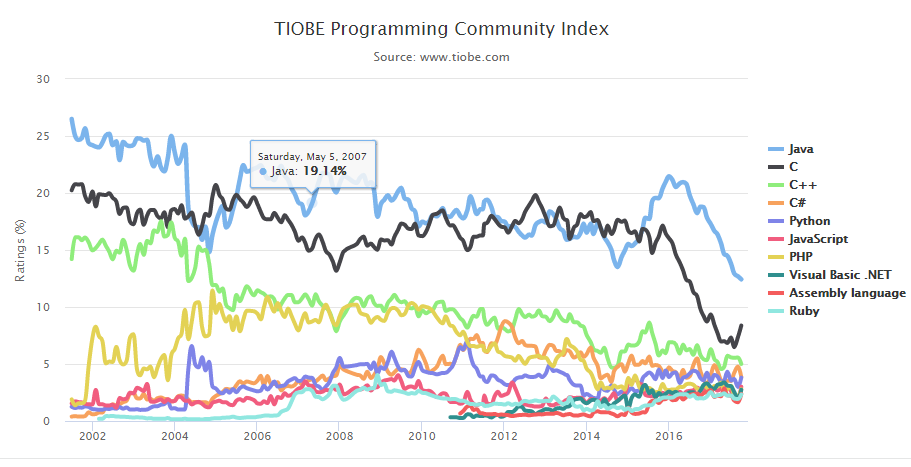
\includegraphics[width=1.0\textwidth]{Java_statics.png}
	\caption{java statics}
    \end{figure}
	\begin{figure}[h]
	\centering
	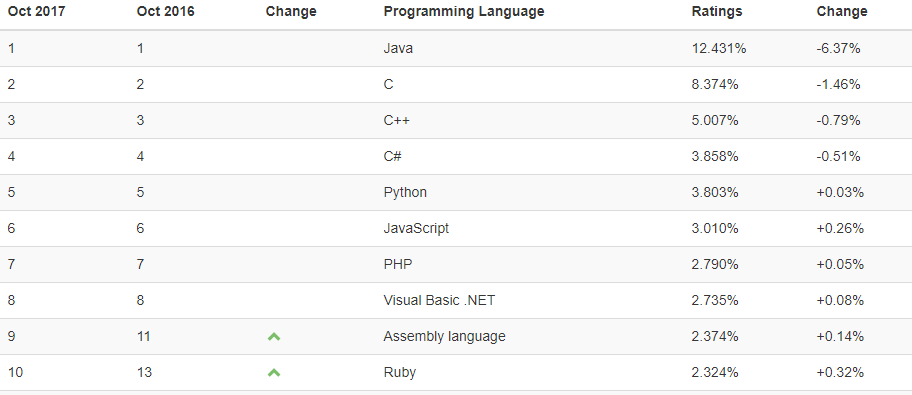
\includegraphics[width=1.0\textwidth]{Java_rank.png}
	\caption{java rank}
    \end{figure}
 As the above statics show, JAVA is the most used language in the industry. Today java it is not an option, it is a requirement for almost all the IT Job Apply. \\Other Major key that push us to use java as language of programming in our project (MassTerInsight) [2] is that the core business of MassTer software [3] is developed using java. As a consequence, it is easy to integrate in our project without any midelware or such web services.
 
\clearpage
\newpage

	\section{Angular JS}
		\begin{figure}[h]
		\centering
		
\includegraphics[width=0.3\textwidth]{AngularJS_logo.png}
		\caption{AngularJS}
	\end{figure}
		\subsection{Introduction}
	AngularJS is a structural framework for dynamic web applications.
	\\
	\\
	It gives to the developers the way to interacte with their html components in ease way instead of using a long javascript code.
	\\
	\\
	The impedance mismatch between dynamic applications and static documents is often solved with:
	\begin{itemize}
		
		\item \textbf{a library} - a collection of functions which are useful when writing web apps. Your code is in charge and it calls into the library when it sees fit. E.g., \colorbox{mygray}{jQuery}.
		\item \textbf{frameworks} - a particular implementation of a web application, where your code fills in the details. The framework is in charge and it calls into your code when it needs something application specific. E.g., \colorbox{mygray}{durandal}, \colorbox{mygray}{ember}, etc.
	\end{itemize}
	AngularJS takes another approach. It attempts to minimize the impedance mismatch between document centric HTML and what an application needs by creating new HTML constructs. AngularJS teaches the browser new syntax through \textbf{directives}. Examples include:
	\begin{itemize}
		\item Data binding, as in \colorbox{mygray}{\{\{\}\}}
		\item DOM control structures for repeating, showing and hiding DOM fragments.
		\item Support for forms and form validation.
		\item Attaching new behavior to DOM elements, such as DOM event handling.
		\item Grouping of HTML into reusable components.	
	\end{itemize}
	\subsection{Features}
	\begin{itemize}
		\item AngularJS is a powerful JavaScript based development framework to create Rich Internet Application(RIA).
		\item AngularJS is a free open source framework.
		\item Large of developers around the world used AngularJS
	\end{itemize}
		Overall, AngularJS is a framework to build large scale and high performance web application while keeping them as easy-to-maintain.
		\\
		\\
		We present in this table the directives used in our project so far.
		\\
		\\
		\begin{table}
				\centering
			\begin{tabular}{|c|p{10cm}|}	
				\hline
				\textbf{Directive} & \textbf{Description }\\
				\hline
				ng-app & tells AngularJS that this is the root element of AngularJS application, we can only have one ng-app directive in the application.
				\\
				ng-model & binds an HTML form element to a variable in the scope  \\
				ng-switch, ng-switch-when & the directive ng-switch lets you hide or show HTML elements depending on an experssion. Child elements with the directive ng-switch-when will be showed up if it gets match, otherwise the element, and its children will be removed.
				\\
				ng-switch-default & define a default section if none of the oher sections get match\\ 
					
				\hline
			\end{tabular} 
		\end{table}
	
	\subsection{Motivation}
	Before starting to use any javascript framework, we have made a research about the most recommended javascript framework.
	\\
	Almost all the articles that I read shows that the most popular frameworks are \colorbox{mygray}{AngularJS}, \colorbox{mygray}{Ember.js}, \colorbox{mygray}{ReactJS} and \colorbox{mygray}{Backbone.js}, AngularJS is the most used framework amongst these frameworks and this is my first motivation.\\
    Based on recent search on Google Trends, the requirements skills  of the industry in all over the world tend  to use more and more the framework AngularJS
	 	\begin{figure}[h]
	 	\centering
	 	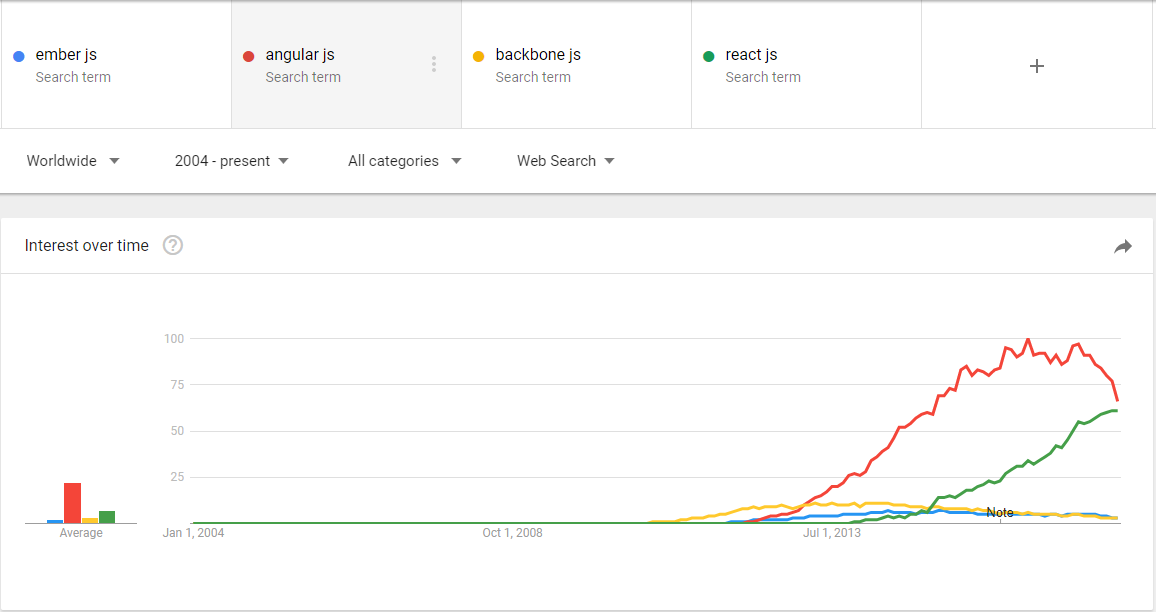
\includegraphics[width=1.0\textwidth]{AngularJS_statics_google_trends.png}
	 	\caption{AngularJS on google trends}
	 \end{figure}
	 

\clearpage
\newpage

	\section{Bootstrap}
	\begin{figure}[h]
		\centering
		
\includegraphics[width=0.20\textwidth]{Boostrap_logo.png}
		\caption{Bootstrap}
	\end{figure}
	\subsection{Introduction}
	\textbf{Bootstrap} is a free and open-source front-end web framework for designing websites and web applications. It contains HTML- and CSS-based design templates for typography, forms, buttons, navigation and other interface components, as well as optional JavaScript plugins. Unlike many web frameworks, it considers front-end development.
	\\
	\\
	Bootstrap was developed by Mark Otto and Jacob Thornton at Twitter, and released as an open source product in August 2011 on GitHub.\\
	In June 2014 Bootstrap was the No.1 project on GitHub!
	\subsection{Features}
	\textbf{Bootstrap 3} supports the latest versions of the \textbf{Google Chrome}, \textbf{Firefox}, \textbf{Internet Explorer}, \textbf{Opera}, and \textbf{Safari} (except on Windows). It additionally supports IE8 and the latest Firefox Extended Support Release (ESR).
	\\
	Since \textbf{2.0}, \textbf{Bootstrap} supports \textbf{responsive web design}. This means the layout of web pages adjusts dynamically, taking into account the characteristics of used device (desktop, tablet, mobile phone).
	\\
	Starting with \textbf{version 3.0}, Bootstrap adopted a mobile-first design philosophy, emphasizing responsive design by default.The \textbf{version 4.0} alpha release added \textbf{Sass} and \textbf{flexbox} support.
	\subsection{Motivation}
	All the research shows that Bootstrap is The most popular HTML, CSS, and JavaScript framework for developing responsive, mobile first projects \\ on the web.
	\\
	According to github, Bootstrap is the second starred repository, with \textbf{115k stars}.
		\begin{figure}[h]
		\centering
		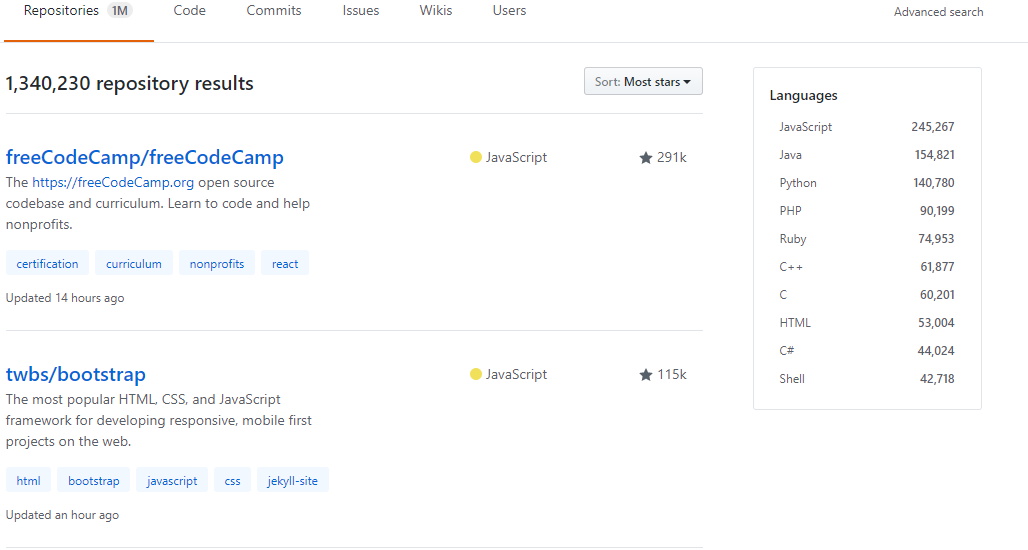
\includegraphics[width=1\textwidth]{Boostrap_statics_github.png}
		\caption{Bootstrap second starred on github}
	\end{figure}

\vspace{66mm}
According to a research in the net, all the high-tech blogs encourage developers to use bootstrap.
\\
\\
 I used a tool offred by google named \textbf{google trends} to make a compraison between subjects in term of most researched.
 \\
 After this compraison in google trends, Bootstrap also is the most googled css framework on the web , compared to the others css frameworks Eg. \textbf{Material UI} which was considered as the most popular css framework after Bootstrap.

\begin{figure}[h]
	\centering
	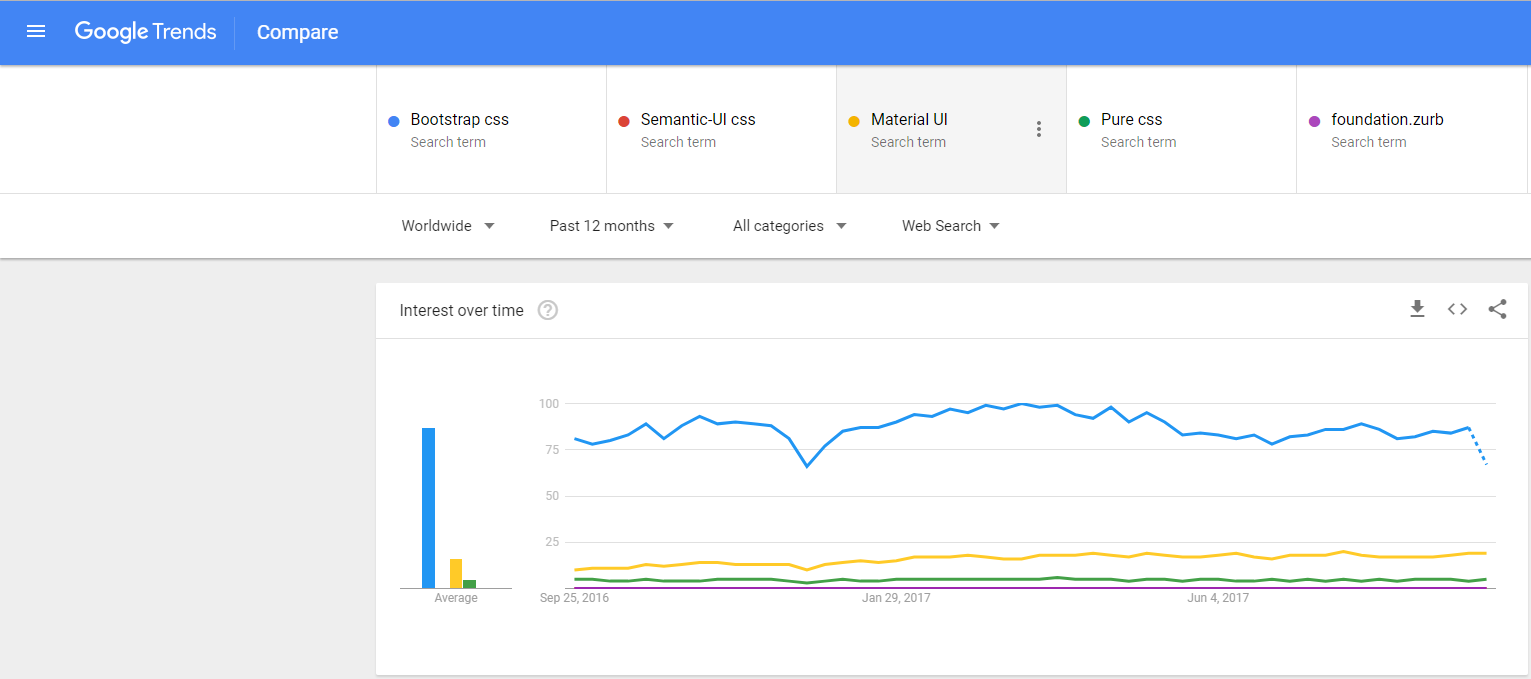
\includegraphics[width=1\textwidth]{Boostrap_statics_google_trends.png}
	\caption{Bootstrap on google trends}
\end{figure}

\clearpage
\newpage


\section{Spring mvc framework}
\begin{figure}[h]
	\centering
	
\includegraphics[width=0.4\textwidth]{Spring_logo.png}
	\caption{Spring MVC}
\end{figure}
\subsection{Introduction}
The Spring Web model-view-controller (MVC) framework is designed around a \colorbox{mygray}{DispatcherServlet} that dispatches requests to handlers, with configurable handler mappings, view resolution, locale, time zone and theme resolution as well as support for uploading files. The default handler is based on the \colorbox{mygray}{@Controller} and \colorbox{mygray}{@RequestMapping} annotations, offering a wide range of flexible handling methods. With the introduction of Spring 3.0, the \colorbox{mygray}{@Controller} mechanism also allows you to create RESTful Web sites and applications, through the \colorbox{mygray}{@PathVariable} annotation and other features.
 \\
\\
Spring’s web MVC framework is, like many other web MVC frameworks, request-driven, designed around a central Servlet that dispatches requests to controllers and offers other functionality that facilitates the development of web applications. Spring’s DispatcherServlet however, does more than just that. It is completely integrated with the Spring IoC container and allows you to use every other feature that Spring has.
\newpage
The request processing workflow of the Spring Web MVC DispatcherServlet is illustrated in the following diagram. The pattern-savvy reader will recognize that the DispatcherServlet is an expression of the ``Front Controlle'' design pattern (this is a pattern that Spring Web MVC shares with many other leading web frameworks).
\begin{figure}[h]
	\centering
	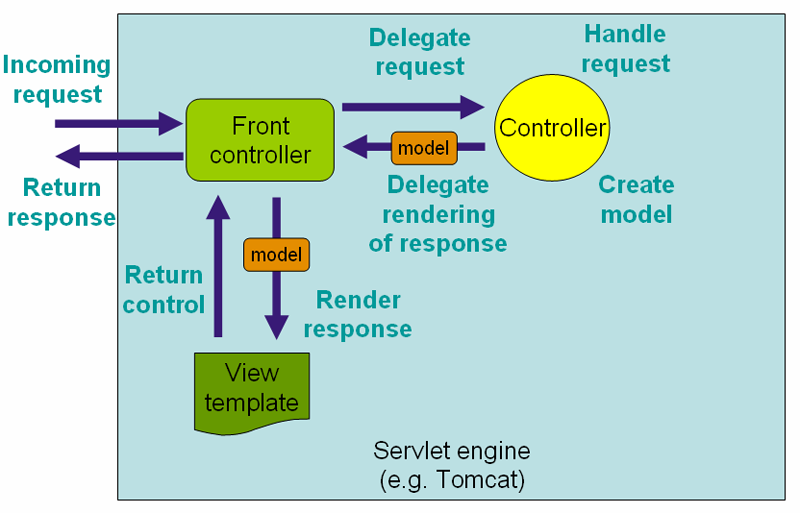
\includegraphics[width=1.1\textwidth]{workflow_spring_mvc.png}
	\caption{The request processing workflow in Spring Web MVC}
\end{figure}

\subsection{Features}
\begin{itemize}
	\item Since Spring MVC framework is designed like any other Spring module, So, it is not necessary to spend any extra time to learn it.
	\item Since all the layers are independent of each others, unit testing can be easier.
	\item Spring framework doesn’t force you to follow any pattern, or implementations to write your business logic. So it gives developer flexibility to implement or integrate any other design pattern to suffice his needs.
	\item Spring provides good separation flexibility between Controller, Service and Data access layers.
	\item Spring provides you with a tag library that is simple and yet very powerful.
	\item View side you can integrate with any UI framework like JSF, Velocity, Freemarker etc.
	\item Supports Annotation based programming along with XML, which makes development faster and cleaner.
	
	We present in this table the annotations used in our project :
	\\
	\\
		\begin{table}
		\centering
		\begin{tabular}{|c|p{10cm}|}
		\hline
		\textbf{Annotation} & \textbf{Description }\\
		\hline
		@Controller & it is responsible for preparing a model Map with data and selecting a view name but it can also write directly to the response stream and complete the request.  \\
		@RequestMapping & it used with method to provide the URI pattern for which handler method will be used.\\
		@RequestBody & the @RequestBody method parameter annotation indcates that a method parameter should be bound to the value of the http request body.  \\
		@ResponseBody & it used to send String response for the web request.  \\	
	    @RequestParam & it used to retrieve the URL parameter and map it to the method argument. \\
		\hline
	\end{tabular}
	\end{table}

\end{itemize}
\newpage
\subsection{Motivation}
According to trusted sources like google engine, yahoo, Linkedin and satckoverflow: sping mvc, struts And JSF are the most JEE frameworks searched and posted by the developers.\\
\begin{figure}[h]

	\centering
	\includegraphics[width=1.0\textwidth]{SpringMVC_statics_google_trends.png}
	\caption{Spring framework on google trends}
	\label{SpringMVC_statics_google_trends}
\end{figure}
\\
The curve of spring mvc in the figure \ref{SpringMVC_statics_google_trends} is very high, wich means that spring is the most used among others frameworks, another key is That spring is the most framework recommend on job application.
\\
\\
The community behind spring is very active.

\clearpage
\newpage

\section{Pivotal tc Server}

\begin{figure}[h]
	
	\centering
	
\includegraphics[width=0.1\textwidth]{icon_tcserver.png}
	\caption{Pivotal tc Server}
	\label{Pivotal tc Server}
\end{figure}

Pivotal tc Server is a open-source Web application server based on Apache Tomcat.
\\
\\
Pivotal tc Server provides :
\begin{itemize}
	\item The best of Apache Tomcat.
	\item Harnesses the power of traditional JEE architectures.
	\item Eliminates the JEE's complexity and performance drawbacks, making it easier, faster.
	\item Pivotal tc Server requires significantly fewer resources than conventional servers.
	\item It is completely compatible with Apache Tomcat.
\end{itemize}

\clearpage
\newpage

\section{Spring Tool Suite}

\begin{figure}[h]
	
	\centering
	
\includegraphics[width=0.15\textwidth]{spring-tool-suite-project-logo.png}
	\caption{spring tool suite}
	\label{spring tool suite}
\end{figure}
\begin{itemize}
	\item The Spring Tool suite is an eclipse-based developing environement that customiwed for developement  Spring applications.
	\item Provides a enviroment to implement, debug, run, and deploy.
	\item It integrates Git,Maven, Pivotal tc Server but also you can use other Web Application Server. 
\end{itemize}

\clearpage
\newpage

\section{Apache Maven}
\begin{figure}[h]
	\centering
	
\includegraphics[width=0.3\textwidth]{Maven_logo.png}
	\caption{Apache Maven}
\end{figure}
Maven is an open-source tool developed by the fondation Apache, which main role is to build projects and the management of libraries used.
\\
\\
Maven provides :
\begin{itemize}
	\item compliation
	\item packaging
	\item dependancy management
	\item deployment
\end{itemize} 

\clearpage
\newpage

\section{HTML5}
\begin{figure}[h]
	\centering
	
\includegraphics[width=0.2\textwidth]{HTML5_logo.png}
	\caption{HTML5}
\end{figure}
HTML5 is the last version of HTML, it comes with new semantics tags (header,aside,...) to divide your page in semantic way, those tags it helps the engine (google, yahoo...) to perform the results. It is easy to learn, compatible with all browsers, now HTML5 replace the falsh, it include tag video, audio, geolocaliton, and more. 
\end{document}